\documentclass[letterpaper,11pt]{article}
\oddsidemargin -1.0cm \textwidth 17.5cm

\usepackage[utf8]{inputenc}
\usepackage[activeacute,spanish, es-lcroman]{babel}
\decimalpoint
\usepackage{amsfonts,setspace}
\usepackage{amsmath}
\usepackage{amssymb, amsmath, amsthm}
\usepackage{comment}
\usepackage{float}
\usepackage{amssymb}
\usepackage{dsfont}
\usepackage{anysize}
\usepackage{multicol}
\usepackage{enumerate}
\usepackage{graphicx}
\usepackage[left=1.5cm,top=2cm,right=1.5cm, bottom=1.7cm]{geometry}
\setlength\headheight{1.5em} 
\usepackage{fancyhdr}
\usepackage{multicol}
\usepackage{hyperref}
\usepackage{wrapfig}
\usepackage{subcaption}
\usepackage{siunitx}
\usepackage{cancel}
\usepackage{mdwlist}
\usepackage{svg}
\pagestyle{fancy}
\fancyhf{}
\renewcommand{\labelenumi}{\normalsize\bfseries P\arabic{enumi}.}
\renewcommand{\labelenumii}{\normalsize\bfseries (\alph{enumii})}
\renewcommand{\labelenumiii}{\normalsize\bfseries \roman{enumiii})}


\begin{document}

\fancyhead[L]{\itshape{Facultad de Ciencias F\'isicas y Matem\'aticas}}
\fancyhead[R]{\itshape{Universidad de Chile}}

\begin{minipage}{11.5cm}
    \begin{flushleft}
        \hspace*{-0.6cm}\textbf{FI1000-1 Introducción a la Física Clásica}\\
        \hspace*{-0.6cm}\textbf{Profesora:} Paulina Lira\\
        \hspace*{-0.6cm}\textbf{Auxiliares:} Alejandro Cartes \& Juan Cristóbal Castro\\
        \hspace*{-0.6cm}\textbf{Ayudantes:} Francisca Bórquez \& Catalina Molina\\
    \end{flushleft}
\end{minipage}

\begin{picture}(2,3)
    \put(366, 10){
\includegraphics[scale=0.9]{2020-1/Imágenes/logo/dfi-fcfm.pdf}}
\end{picture}

\begin{center}
	\LARGE\textbf{Ejercicio \#3}
\end{center}

\vspace{-1cm}
\begin{enumerate}\setlength{\itemsep}{0.4cm}

\rfoot[]{pág. \thepage}

\item[]

\item En un día lluvioso sin viento, en donde las gotas caen verticalmente a velocidad constante con respecto a la Tierra, pasa un tren a una rapidez $v_0$. Los pasajeros del tren constatan que las gotas de lluvia dejan huellas en las ventanas laterales inclinadas en un ángulo de $60^{\circ}$ con respecto a la vertical. Determine la \textbf{velocidad}~(dirección y magnitud) de la lluvia en relación:

\begin{multicols}{2}
\begin{enumerate}
    \item al tren
    \item a la Tierra
\end{enumerate}
\end{multicols}

\textbf{Nota:} $\sin{(60^{\circ})}=\sqrt{3}/2$ y $\cos{(60^{\circ})}=1/2$

\begin{figure}[H]
    \centering
    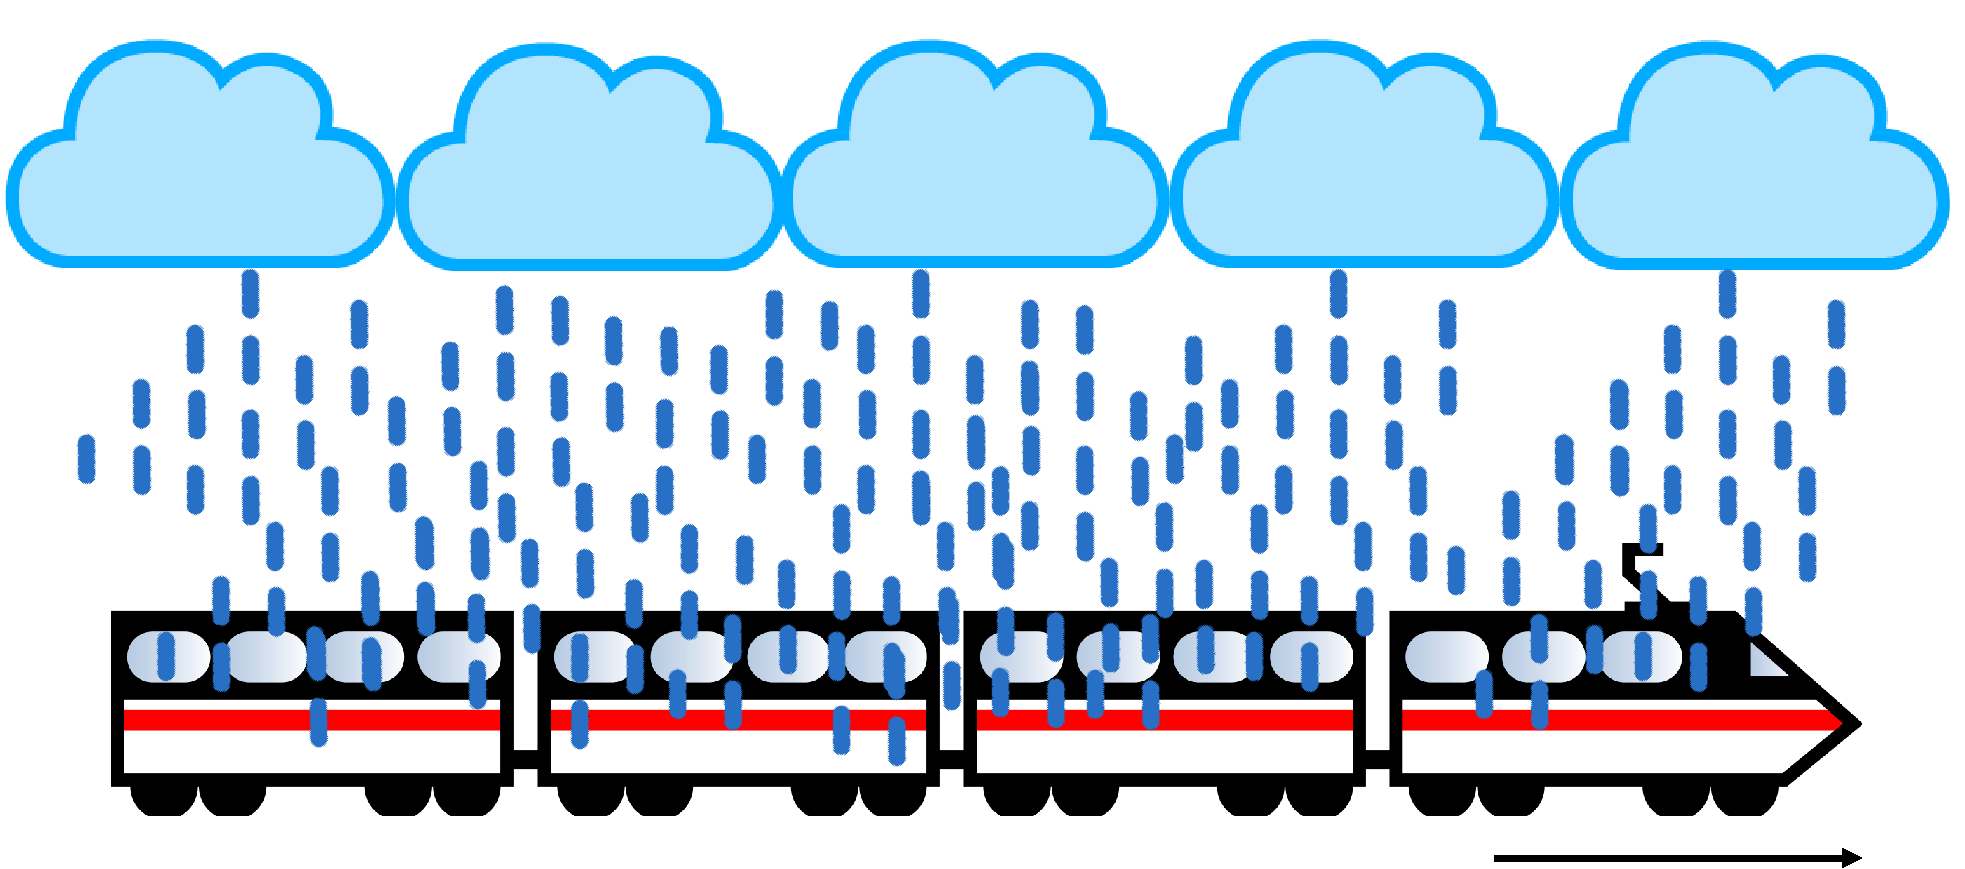
\includegraphics[width=0.6\linewidth]{2021-1/Imagenes/ejercicios/tren.pdf}
\end{figure}
\end{enumerate}

\end{document}